\documentclass[oneside,openany]{book}

\usepackage{graphicx}
\usepackage[dvipsnames]{xcolor}
\usepackage{hyperref}
\usepackage{amsmath,amssymb}
\usepackage[toc,page]{appendix}
\usepackage{booktabs}
\usepackage{array}
\usepackage{caption}
\usepackage{enumitem}
\usepackage{tikz}
\usepackage{pgfplots}
\pgfplotsset{compat=1.18}
\usetikzlibrary{arrows.meta,positioning,shapes.geometric,fit,backgrounds,calc}

\hypersetup{colorlinks=true,linkcolor=black,citecolor=black,urlcolor=blue}

\renewcommand{\baselinestretch}{1}

\setlength{\textheight}{9in}
\setlength{\textwidth}{6.5in}
\setlength{\headheight}{0in}
\setlength{\headsep}{0in}
\setlength{\topmargin}{0in}
\setlength{\oddsidemargin}{0in}
\setlength{\evensidemargin}{0in}
\setlength{\parindent}{.3in}
\pagestyle{plain}

% ---- Tighten float spacing and reduce blank space (format preserved) ----
\setlength{\textfloatsep}{10pt plus 2pt minus 2pt}
\setlength{\intextsep}{10pt plus 2pt minus 2pt}
\setlength{\floatsep}{10pt plus 2pt minus 2pt}
\renewcommand{\topfraction}{0.92}
\renewcommand{\bottomfraction}{0.85}
\renewcommand{\textfraction}{0.06}
\renewcommand{\floatpagefraction}{0.72}
\captionsetup{font=small,skip=4pt}

% ---- Colour palette (consistent across all figures) ----
\definecolor{cdone}{HTML}{2E7D32}
\definecolor{cdoneD}{HTML}{1B5E20}
\definecolor{cnow}{HTML}{F9A825}
\definecolor{cnowD}{HTML}{F57F17}
\definecolor{ctodo}{HTML}{CFD8DC}
\definecolor{ctodoD}{HTML}{90A4AE}
\definecolor{cprob}{HTML}{FFCDD2}
\definecolor{cprobD}{HTML}{E53935}
\definecolor{cgood}{HTML}{C8E6C9}
\definecolor{cgoodD}{HTML}{43A047}
\definecolor{cball}{HTML}{E3F2FD}
\definecolor{cballD}{HTML}{1976D2}
\definecolor{cours}{HTML}{EDE7F6}
\definecolor{coursD}{HTML}{7E57C2}
\definecolor{cstep}{HTML}{E3F2FD}
\definecolor{cwarn}{HTML}{EF6C00}

% ---- Shared TikZ node styles ----
\tikzset{
  fbox/.style={draw, rounded corners, align=center, inner sep=4pt,
               minimum height=8.5mm, font=\footnotesize},
  ndone/.style={fbox, fill=cdone, text=white, draw=cdoneD, line width=0.8pt},
  nnow/.style={fbox, fill=cnow, text=black, draw=cnowD, line width=1.2pt},
  ntodo/.style={fbox, fill=ctodo, text=black, draw=ctodoD},
  nprob/.style={fbox, fill=cprob, text=cprobD, draw=cprobD},
  ngood/.style={fbox, fill=cgood, text=cdoneD, draw=cgoodD},
  nball/.style={fbox, fill=cball, text=cballD, draw=cballD},
  nours/.style={fbox, fill=cours, text=coursD, draw=coursD},
  nstep/.style={fbox, fill=cstep, text=cballD, draw=cballD},
  nneu/.style={fbox, fill=black!6, text=black, draw=black!40},
  flow/.style={-{Latex[length=2mm]}, line width=0.7pt},
  flowd/.style={-{Latex[length=2mm]}, line width=0.7pt, dashed},
}

\begin{document}
\bibliographystyle{plain}

\large

% =====================================================================
% COVER PAGE
% =====================================================================
\thispagestyle{empty}
\centerline{\bf A REPORT}
\vspace*{0.3cm}
\centerline{\bf ON}
\vspace*{0.3cm}
\centerline{\bf 3D HUMAN POSE ESTIMATION FOR CRICKET BROADCASTING}
\vspace*{0.2cm}
\centerline{\normalsize\it Multi-camera pose for broadcast stories and Unreal Engine animation}
\vspace*{1.1cm}

\centerline{BY}
\vspace*{0.6cm}

\begin{center}
	\begin{tabular}{lll}
		Name of the student & \hspace*{1cm} ID No. & \hspace*{1cm} Discipline \\
		Aksh Shah &\hspace*{1cm} 2024A7PS0532G &\hspace*{1cm} B.E. Computer Science \\
	\end{tabular}
\end{center}

\vspace*{1.1cm}
\begin{center}
	{\bf Prepared in partial fulfilment of the \\
	Practice School - I Course} \\
\end{center}

\vspace*{0.4cm}

\centerline{AT}

\vspace*{0.6cm}
        \centerline{\bf Quidich Innovation Labs, Mumbai}
	\vspace{0.2cm}
	\centerline{\bf A Practice School - I}
	\vspace{0.2cm}
	\centerline{\bf Station of}
	\vspace{0.4cm}
\begin{center}

\includegraphics[width=1.0in]{figures/logo.pdf}
\end{center}
	\vspace{0.3cm}

	\centerline{\bf BIRLA INSTITUTE OF TECHNOLOGY \& SCIENCE, PILANI}
	\vspace*{0.3cm}
	\centerline{\bf (K. K. Birla Goa Campus)}
	\vspace*{0.4cm}
	\centerline{\bf June, 2026}
	\newpage

% =====================================================================
% ABSTRACT SHEET
% =====================================================================
\thispagestyle{empty}

	\centerline{\bf BIRLA INSTITUTE OF TECHNOLOGY \& SCIENCE, PILANI}
	\vspace*{0.2cm}
	\centerline{\bf Practice School Division}
	\vspace*{0.3cm}
	{\normalsize
		\setlength{\extrarowheight}{2pt}
		\begin{tabular}{p{6.2cm}p{9.3cm}}
			Station: Quidich Innovation Labs & \hspace*{0.5cm} Centre: Remote (Online) \\[7pt]
			Duration: 8 weeks &\hspace*{0.5cm} Date of start: 25 May 2026 \\[7pt]
			Date of submission: 20 June 2026 & {} \\[7pt]
			\multicolumn{2}{p{15.5cm}}{Title of the project: 3D Human Pose Estimation for
			Cricket Broadcasting (multi-camera pose for broadcast stories and Unreal Engine
			animation).} \\[7pt]
			\multicolumn{2}{p{15.5cm}}{ID No., Name and Discipline of the student:
			2024A7PS0532G, Aksh Shah, B.E. Computer Science.} \\[7pt]
			\multicolumn{2}{p{15.5cm}}{Name and Designation of the expert: Ms. Simone Singh,
			Mentor, Quidich Innovation Labs.} \\[7pt]
			\multicolumn{2}{p{15.5cm}}{Name of the PS faculty member: Prof. Tarkeshwar Singh,
			Associate Professor, Department of Mathematics, BITS Pilani K. K. Birla Goa
			Campus.} \\[7pt]
			\multicolumn{2}{p{15.5cm}}{Key words: human pose estimation, multi-camera
			triangulation, re-identification, cricket broadcast analytics, model
			benchmarking.} \\[7pt]
			\multicolumn{2}{p{15.5cm}}{Project areas: computer vision, sports broadcast
			technology, applied machine learning.} \\[7pt]
			\multicolumn{2}{p{15.5cm}}{Abstract: This report documents the first half of a
			Practice School project at Quidich Innovation Labs on real-time 3D human pose
			estimation for cricket broadcast. The first two weeks established the technical
			foundations of 2D and 3D pose estimation and produced an audited survey of more
			than fifty pose models released after 2020, framed around the speed against
			accuracy trade-off that governs live broadcast use. The third week turned that
			survey into a reproducible benchmarking repository with a single measurement
			protocol. The fourth week applied this foundation to a real seven-camera
			calibrated cricket capture: a foundation-readiness audit (Phase 0) and a
			per-camera person detection and 2D pose stage (Phase 1) were completed and
			verified on a full delivery. The report closes with a quantified account of the
			remaining work for the second half, beginning with per-camera tracking and
			progressing to cross-camera re-identification, role assignment, and smooth 3D
			reconstruction for downstream story creation and Unreal Engine rendering.} \\[12pt]
			
\includegraphics[height=1.0cm]{figures/sign_trim.png} & \\[-2pt]
			Signature of the student & \hspace*{1cm}Signature of the PS faculty member \\[5pt]
			Date: 20 June 2026 & \hspace*{1cm}Date: \\
		\end{tabular}}

	\newpage

% =====================================================================
% ACKNOWLEDGEMENTS
% =====================================================================
	\centerline{\bf \Large Acknowledgements}
	\vspace*{0.5cm}
		\par\noindent I thank Quidich Innovation Labs for the opportunity to work on a live
		sports broadcast problem and for access to the calibrated multi-camera cricket data
		and the existing ball-tracking pipeline that this project builds upon. I am grateful
		to my company mentor, Ms. Simone Singh, for technical guidance and for framing the
		problem in production terms.

		\par\noindent I thank my Practice School faculty in-charge, Prof. Tarkeshwar Singh, and
		the BITS Pilani Practice School Division for their supervision and feedback during the
		first half of the programme. I also acknowledge my project teammates for the
		collaborative discussions that shaped the group's shared design, while noting that the
		implementation and analysis presented in this individual report are my own
		contribution.

		\vspace*{1.2cm}
		\par\noindent 
\includegraphics[height=1.1cm]{figures/sign_trim.png}
		\par\noindent {\bf Signature of the student} \\
		{\bf Date:} 20 June 2026

\tableofcontents
\listoffigures
\listoftables

% =====================================================================
\chapter{Introduction}
% =====================================================================

\section{Organisation and project context}
Quidich Innovation Labs is a sports broadcast technology company. It builds the systems that
turn raw match footage into the graphics and analytical segments that viewers see during a
live cricket broadcast. One established product line is Decision Review System (DRS) style
ball tracking, in which several calibrated cameras observe a single moving ball, its position
is reconstructed in three dimensions, and the reconstruction is rendered as a broadcast
graphic. This Practice School project extends that established idea from a single ball point to
full human players.

The eventual goal of the project is \textbf{real-time three dimensional (3D) human pose
estimation} for cricket broadcast. A \emph{pose} is the set of positions of a person's body
joints, such as the shoulders, elbows, knees, and ankles. A \emph{2D pose} gives those joints
on the flat image plane of one camera. A \emph{3D pose} gives them in real world space, which
is what is needed to drive broadcast graphics and biomechanical analysis. The output of the
work is intended to be consumed in two forms: a structured data file describing each player's
joints over time, and a clean, rigged animation that can be rendered inside Unreal Engine, the
game engine used for broadcast visualisation.

\section{Why body pose matters: events and stories}
A cricket broadcast is organised around \emph{events} and \emph{stories}. An event is a single
passage of play, for example a delivery that results in a wide, a no-ball, a run-out, or a
wicket. A story is a short explanatory or analytical segment built around an event. Many of the
most valuable stories cannot be told from ball tracking alone, because they depend on where a
player's body is. Table~\ref{tab:stories} lists representative examples taken from the
project's story catalogue, each of which requires body pose rather than the ball alone.

\begin{table}[!h]
	\begin{center}
		\caption{Representative broadcast stories that require human body pose. Source: the
		project's internal story catalogue.}
		\label{tab:stories}
		\footnotesize
		\begin{tabular}{p{3.4cm}p{4.0cm}p{6.6cm}}
			\toprule
			\textbf{Story} & \textbf{Key body landmarks} & \textbf{What the pose adds} \\
			\midrule
			Waist-high full toss (no-ball) & Batter waist, shoulders, head & Estimates where the
			batter's waist would be standing upright and checks whether the ball passed above it. \\
			Front-foot no-ball & Bowler front foot & Pinpoints, frame by frame, exactly where the
			bowler's front foot lands relative to the popping crease. \\
			Wide ball decision & Batter feet, hips, shoulder, lead arm & Tracks how far the batter
			can reach and whether the batter moved toward or away from the ball. \\
			Stumping or run-out & Batter feet, bat tip & Locates the foot and bat at the instant the
			bails are dislodged to judge whether the ground was made in time. \\
			LBW impact distance & Batter feet, pads & Measures how far from the stumps the ball
			struck the pads, which affects the reliability of the decision. \\
			Bowler release mechanics & Wrist, shoulder, jump foot, stride & Reveals the body
			mechanics behind extra pace or a disguised slower ball. \\
			\bottomrule
		\end{tabular}
	\end{center}
\end{table}

These stories explain why accurate, stable body pose is a foundational capability for the
broadcaster. The pose data feeds two distinct downstream consumers: an analytics layer that
composes the stories, and a rendering layer that animates the player in Unreal Engine.
Figure~\ref{fig:valuechain} shows this value chain.

\begin{figure}[ht]
\begin{center}
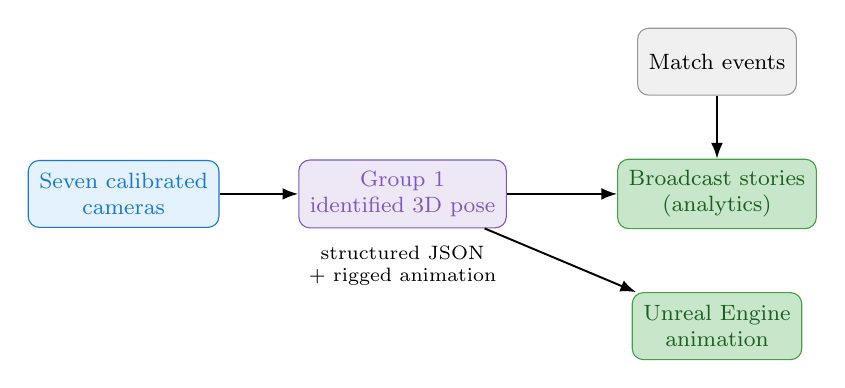
\begin{tikzpicture}[node distance=6mm and 10mm]
  \node[nball] (cam) {Seven calibrated\\cameras};
  \node[nours, right=of cam] (g1) {Group 1\\identified 3D pose};
  \node[ngood, right=14mm of g1] (stories) {Broadcast stories\\(analytics)};
  \node[ngood, below=8mm of stories] (ue) {Unreal Engine\\animation};
  \node[nneu, above=8mm of stories] (events) {Match events};
  \draw[flow] (cam) -- (g1);
  \draw[flow] (g1) -- (stories);
  \draw[flow] (g1) -- (ue);
  \draw[flow] (events) -- (stories);
  \node[font=\scriptsize, below=1mm of g1, text width=3.2cm, align=center]
    {structured JSON \\ + rigged animation};
\end{tikzpicture}
\caption{The broadcast value chain. Calibrated cameras feed Group 1, which produces identified
3D pose. That pose, combined with match events, drives broadcast stories and is also rendered as
an Unreal Engine animation.}
\label{fig:valuechain}
\end{center}
\end{figure}

\section{Team structure and individual scope}
The broader project is divided across three groups whose work is interdependent, summarised in
Table~\ref{tab:groups}. Group 1 is the perception and geometry layer: it turns camera footage
into identified, role-labelled, smooth 3D skeletons. Group 2 composes the broadcast stories,
and Group 3 interprets the cricket event. Groups 2 and 3 both depend on Group 1's output.

\begin{table}[!h]
	\begin{center}
		\caption{The three project groups and their dependencies.}
		\label{tab:groups}
		\footnotesize
		\begin{tabular}{p{1.6cm}p{6.4cm}p{6.0cm}}
			\toprule
			\textbf{Group} & \textbf{Responsibility} & \textbf{Relationship} \\
			\midrule
			Group 1 & Player re-identification, role assignment, multi-camera tracking, and clean
			3D pose. & Supplies pose data to Groups 2 and 3 and animation to Unreal Engine. \\
			Group 2 & Story creation. & Consumes Group 1 pose and Group 3 events. \\
			Group 3 & Interpretation of the complete cricket event. & Supplies event understanding
			to Group 2. \\
			\bottomrule
		\end{tabular}
	\end{center}
\end{table}

This report concerns my individual work within Group 1. Group 1 work is necessarily
collaborative, and where group context is needed it is described accurately, but the audit,
benchmarking, implementation, and analysis presented here as completed work are my own
contribution. The remaining phases are distributed across the team; the specific ownership of
future phases is stated in Chapter~\ref{ch:conclusions} only to make the plan concrete.

\section{The capture setup and the core challenge}
The cricket data is produced by a rig of seven synchronised, calibrated cameras arranged around
the pitch, the same class of rig Quidich uses for ball tracking. Because each camera is
calibrated into one shared world coordinate system, a joint that is seen by several cameras can
be combined into a single 3D point by a geometric procedure called \emph{triangulation}.

The central engineering challenge is not simply detecting poses in one image. It is preserving
each player's identity across all seven views and over time, and producing 3D motion that is
stable and smooth enough to render on broadcast, despite noise, occlusion, missing views, and
geometric error. Chapters~\ref{ch:litreview} to \ref{ch:results} describe how the first four
weeks built toward this goal, and Chapter~\ref{ch:conclusions} sets out the remaining work.

% =====================================================================
\chapter{Literature Review}
\label{ch:litreview}
% =====================================================================
The first two weeks were a structured study of human pose estimation and a survey of the
available models, motivated by a single practical question: which pose estimation model should
the project adopt. This chapter records that study and the audited survey it produced.

\section{From 2D images to 3D pose}
A single camera produces a flat image and therefore cannot, on its own, recover true depth.
Two image points that lie on the same line of sight project to the same pixel, so depth is
ambiguous from one view. The standard solution is multiple calibrated cameras
\cite{hartley2004multiview}. When the same joint is detected in two or more calibrated views,
the lines of sight from each camera intersect at a single point in space, and that intersection
is the 3D position of the joint. This is triangulation. With more cameras the estimate becomes
more robust, because a joint hidden in one view may still be visible in others.
Figure~\ref{fig:2dto3d} shows the path from per-camera 2D joints to a clean 3D animation.

\begin{figure}[ht]
\begin{center}
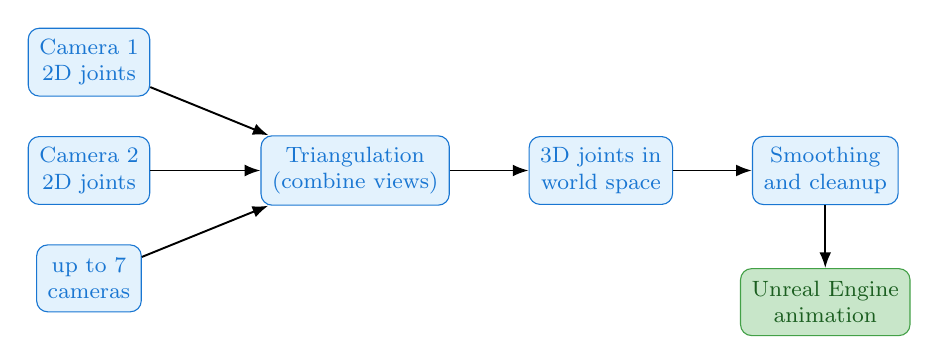
\begin{tikzpicture}[node distance=5mm and 9mm]
  \node[nball] (c1) {Camera 1\\2D joints};
  \node[nball, below=of c1] (c2) {Camera 2\\2D joints};
  \node[nball, below=of c2] (c3) {up to 7\\cameras};
  \node[nstep, right=14mm of c2] (tri) {Triangulation\\(combine views)};
  \node[nstep, right=10mm of tri] (j3) {3D joints in\\world space};
  \node[nstep, right=10mm of j3] (sm) {Smoothing\\and cleanup};
  \node[ngood, below=8mm of sm] (ue) {Unreal Engine\\animation};
  \draw[flow] (c1) -- (tri);
  \draw[flow] (c2) -- (tri);
  \draw[flow] (c3) -- (tri);
  \draw[flow] (tri) -- (j3);
  \draw[flow] (j3) -- (sm);
  \draw[flow] (sm) -- (ue);
\end{tikzpicture}
\caption{The route from 2D pose in each camera to a smooth 3D animation. Triangulation combines
calibrated views into 3D joints, which are then cleaned and smoothed before export.}
\label{fig:2dto3d}
\end{center}
\end{figure}

\section{The speed against accuracy trade-off}
Pose models occupy a spectrum between two extremes. At one end are large, highly accurate
models such as Meta's Sapiens family \cite{khirodkar2024sapiens}, which produce detailed
skeletons but run far too slowly for live broadcast. At the other end are small models that run
at hundreds of frames per second but miss joints, particularly when players overlap or are
partly hidden. Live cricket requires neither extreme. It requires a middle ground: a model fast
enough for real-time use yet accurate enough that the reconstructed 3D skeleton is correct.
Figure~\ref{fig:quadrant} positions representative models on this trade-off and marks the region
of interest.

\begin{figure}[ht]
\begin{center}
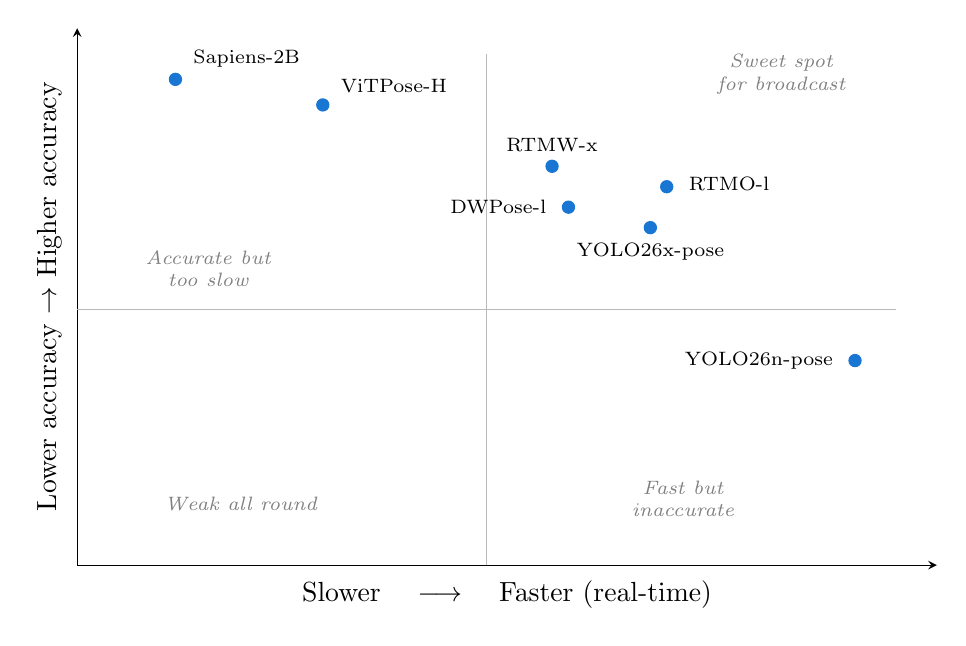
\begin{tikzpicture}
\begin{axis}[
  width=12.5cm, height=8.4cm,
  xlabel={Slower \quad $\longrightarrow$ \quad Faster (real-time)},
  ylabel={Lower accuracy $\rightarrow$ Higher accuracy},
  xmin=0, xmax=1.05, ymin=0, ymax=1.05,
  xtick=\empty, ytick=\empty,
  axis lines=left, clip=false,
]
  % quadrant dividers, crossing cleanly at the centre (0.5, 0.5)
  \draw[gray!55] (axis cs:0.5,0) -- (axis cs:0.5,1.0);
  \draw[gray!55] (axis cs:0,0.5) -- (axis cs:1.0,0.5);
  % one descriptor per quadrant, kept clear of the markers
  \node[gray, font=\itshape\scriptsize, align=center] at (axis cs:0.86,0.96) {Sweet spot\\for broadcast};
  \node[gray, font=\itshape\scriptsize, align=center] at (axis cs:0.16,0.58) {Accurate but\\too slow};
  \node[gray, font=\itshape\scriptsize, align=center] at (axis cs:0.20,0.12) {Weak all round};
  \node[gray, font=\itshape\scriptsize, align=center] at (axis cs:0.74,0.13) {Fast but\\inaccurate};
  % models (coordinates mirror the original survey chart)
  \addplot[only marks, mark=*, mark size=2.2pt, draw=cballD, fill=cballD] coordinates {
    (0.12,0.95) (0.30,0.90) (0.58,0.78) (0.60,0.70) (0.72,0.74) (0.70,0.66) (0.95,0.40)};
  \node[font=\scriptsize, anchor=south west] at (axis cs:0.13,0.955) {Sapiens-2B};
  \node[font=\scriptsize, anchor=south west] at (axis cs:0.31,0.905) {ViTPose-H};
  \node[font=\scriptsize, anchor=south] at (axis cs:0.58,0.79) {RTMW-x};
  \node[font=\scriptsize, anchor=east] at (axis cs:0.585,0.70) {DWPose-l};
  \node[font=\scriptsize, anchor=west] at (axis cs:0.735,0.745) {RTMO-l};
  \node[font=\scriptsize, anchor=north] at (axis cs:0.70,0.648) {YOLO26x-pose};
  \node[font=\scriptsize, anchor=east] at (axis cs:0.935,0.40) {YOLO26n-pose};
\end{axis}
\end{tikzpicture}
\caption{Speed against accuracy for representative pose models. Positions are an illustrative
summary of the audited survey, not exact benchmark coordinates; the underlying numbers are in
Tables~\ref{tab:bodymodels} and \ref{tab:wbmodels} and Appendix~\ref{app:models}.}
\label{fig:quadrant}
\end{center}
\end{figure}

\section{How the metrics are read}
Comparing models requires a shared vocabulary of metrics. Table~\ref{tab:glossary} defines the
ones used throughout this report in plain terms. A recurring caveat documented during the survey
is that these numbers are only comparable when models are tested on the \emph{same dataset and
hardware}. For example, the 17-joint COCO benchmark \cite{lin2014coco}, the 133-joint
COCO-WholeBody benchmark \cite{jin2020wholebody}, and the separate 308-joint test used by the
Sapiens v2 family are different protocols, so their scores must not be compared head to head.

\begin{table}[!h]
	\begin{center}
		\caption{Plain-language glossary of the pose metrics used in this report.}
		\label{tab:glossary}
		\footnotesize
		\begin{tabular}{p{2.6cm}p{7.6cm}p{3.6cm}}
			\toprule
			\textbf{Term} & \textbf{Meaning} & \textbf{Why it matters} \\
			\midrule
			AP (AP50-95) & Average Precision: how often predicted joints land close to the truth,
			averaged over strict to loose tolerances. Higher is better. & Standard accuracy score
			for 2D pose. \\
			MPJPE & Mean Per Joint Position Error, in millimetres: average distance between a
			predicted 3D joint and its true location. Lower is better. & Standard accuracy score
			for 3D pose. \\
			FPS & Frames per second the model can process. & Decides whether it can run live. \\
			Latency (ms) & Time to process one frame. Lower is better. & The frame-by-frame
			real-time constraint. \\
			Params / GFLOPs & Model size and compute per frame. & Proxy for hardware cost and
			deployability. \\
			\bottomrule
		\end{tabular}
	\end{center}
\end{table}

\section{The surveyed models}
The survey catalogued more than fifty model variants across two families: dense
\emph{whole-body} models that estimate the body together with hands, feet, and face, and lighter
\emph{body-only} models that estimate the seventeen main joints. Every figure in the audited
tables is backed by an official paper, repository, or model card, with conflicting published
numbers flagged rather than silently averaged. This audit was consolidated into two internal
production-focused review documents that underpin the conclusions in this chapter
\cite{prodreview_centric,prodreview_comparative}. Tables~\ref{tab:bodymodels} and
\ref{tab:wbmodels} present a verified, condensed slice; the extended table is in
Appendix~\ref{app:models}.

\begin{table}[!h]
	\begin{center}
		\caption{Body-centric, real-time pose candidates (condensed from the audited survey).}
		\label{tab:bodymodels}
		\footnotesize
		\begin{tabular}{p{2.6cm}p{2.4cm}p{3.0cm}p{1.8cm}p{3.2cm}}
			\toprule
			\textbf{Model} & \textbf{Accuracy (COCO AP)} & \textbf{Speed} & \textbf{Size} &
			\textbf{Why it is of interest} \\
			\midrule
			YOLO26x-pose \cite{ultralytics_pose} & 71.6 AP & about 82 FPS on T4 (12.2 ms) & 57.6M
			params & Newest YOLO pose head; broad export to ONNX, TensorRT, CoreML. \\
			RTMO-l \cite{lu2023rtmo} & 74.8 AP; CrowdPose-Hard 65.3 & 141 FPS on V100 & 44.8M
			params & One-stage; cost does not grow with player count; strong under occlusion. \\
			RTMPose-l \cite{jiang2023rtmpose} & 75.8 AP & TensorRT-FP16 3.46 ms per crop & 27.7M
			params & Very fast per person; mobile friendly. \\
			ViTPose-H \cite{xu2022vitpose} & 79.1 AP & 241 FPS on A100 (batch 64) & 632M params &
			Accuracy ceiling for 2D body; heavy. \\
			\bottomrule
		\end{tabular}
	\end{center}
\end{table}

\begin{table}[!h]
	\begin{center}
		\caption{Dense whole-body pose candidates (condensed from the audited survey).}
		\label{tab:wbmodels}
		\footnotesize
		\begin{tabular}{p{2.6cm}p{3.4cm}p{2.2cm}p{4.6cm}}
			\toprule
			\textbf{Model} & \textbf{Accuracy (Whole-body AP)} & \textbf{Size} &
			\textbf{Why it is of interest} \\
			\midrule
			DWPose-l \cite{yang2023dwpose} & 66.5 (384x288) & about 4.5M params & Trained to infer
			hidden joints; good under occlusion. \\
			RTMW-x \cite{jiang2024rtmw} & 70.2 (384x288) & mid-size & Best balance of whole-body
			detail and speed. \\
			Sapiens-2B \cite{khirodkar2024sapiens} & 74.4 & 2.16B params & Highest open whole-body
			accuracy; offline only. \\
			\bottomrule
		\end{tabular}
	\end{center}
\end{table}

The clearest conclusion from the survey is that dense whole-body models substantially improve
suitability for cricket, because they capture the wrists at ball release and the feet for
no-ball calls, but the strongest dense models give up real-time speed unless the pipeline is
carefully staged. The body-only family, led by RTMO and the YOLO pose heads
\cite{maji2022yolopose}, offers practical real-time operation at the cost of finer whole-body
detail. A recent systematic review of
real-time pose estimation reaches a consistent conclusion about this staging trade-off
\cite{posereview2025}. These findings directly informed the model recommendations in
Chapter~\ref{ch:recommendations} and the baseline choice in Chapter~\ref{ch:methodology}.

% =====================================================================
\chapter{Methodology}
\label{ch:methodology}
% =====================================================================
This chapter describes the methodology of the third and fourth weeks: first the benchmarking
repository that makes all later experiments comparable, then the Group 1 pipeline design and the
methodology of the two phases completed on the real cricket data.

\section{The benchmarking repository (Week 3)}
The survey produced numbers collected from published sources. To compare any model the team
tests in future, those tests must be run the same way, on the same metrics, with full record of
the hardware and software used. Without a fixed protocol, two people testing two models would
produce numbers that cannot be compared. The third week therefore turned the survey into a
benchmarking repository: shared code and a single fixed protocol so that every later result is
reproducible and directly comparable.

The repository is driven from configuration files that act as the single source of truth for
which models, datasets, metrics, and skeletons exist. A single command line tool runs a
five-stage pipeline, shown in Figure~\ref{fig:bench}: \texttt{prepare} fetches and checks data,
\texttt{smoke} runs a one-image readiness check per model, \texttt{run} executes the benchmark,
\texttt{aggregate} collates the per-run outputs, and \texttt{report} produces the comparison
tables. Each run writes a small, timestamped folder containing its metrics together with
hardware and software manifests, so that two contributors never conflict and every number is
traceable to the exact conditions that produced it. To avoid drawing speed conclusions from
incompatible setups, each model runs in its own isolated software environment, and the
repository records that laptops are for functional validation rather than speed conclusions.

\begin{figure}[ht]
\begin{center}
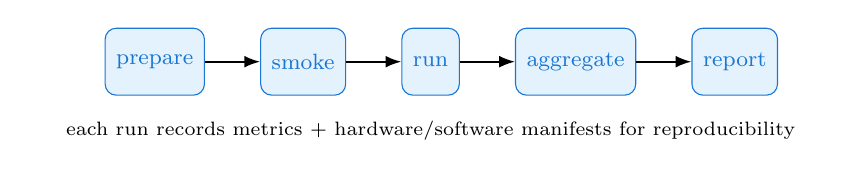
\begin{tikzpicture}[node distance=7mm]
  \node[nstep] (p) {prepare};
  \node[nstep, right=of p] (s) {smoke};
  \node[nstep, right=of s] (r) {run};
  \node[nstep, right=of r] (a) {aggregate};
  \node[nstep, right=of a] (rep) {report};
  \draw[flow] (p)--(s); \draw[flow] (s)--(r); \draw[flow] (r)--(a); \draw[flow] (a)--(rep);
  \node[font=\scriptsize, below=2mm of r, text width=10cm, align=center]
    {each run records metrics + hardware/software manifests for reproducibility};
\end{tikzpicture}
\caption{The five-stage benchmarking pipeline. Configuration files are the source of truth, and
every run is recorded with full metadata so results are comparable across people and machines.}
\label{fig:bench}
\end{center}
\end{figure}

\section{Group 1 pipeline design (Week 4)}
With real cricket data available, the Group 1 task was decomposed into eight phases, P0 to P7,
ordered by dependency rather than by calendar. Figure~\ref{fig:phases} shows the full pipeline
and marks the two phases completed in Week 4. The guiding design principle is \emph{geometry
first}: because both teams wear near-identical kits, appearance alone cannot reliably tell
players apart, so the calibrated camera geometry is used as the primary signal for association
and 3D reconstruction.

\begin{figure}[ht]
\begin{center}
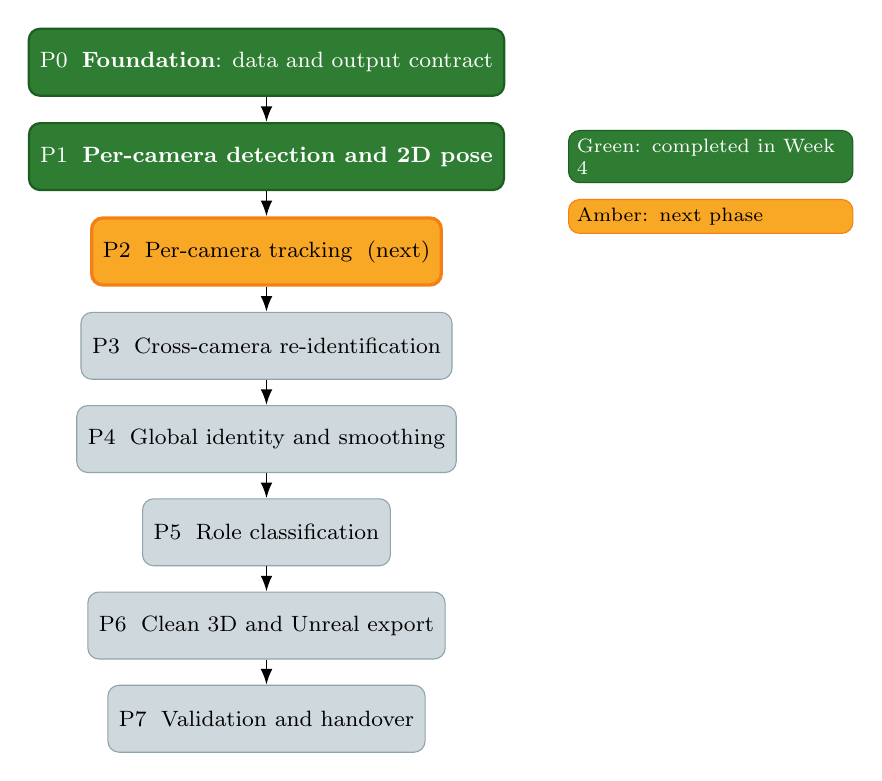
\begin{tikzpicture}[node distance=3.2mm]
  \node[ndone] (p0) {P0 \;\textbf{Foundation}: data and output contract};
  \node[ndone, below=of p0] (p1) {P1 \;\textbf{Per-camera detection and 2D pose}};
  \node[nnow, below=of p1] (p2) {P2 \;Per-camera tracking \;(next)};
  \node[ntodo, below=of p2] (p3) {P3 \;Cross-camera re-identification};
  \node[ntodo, below=of p3] (p4) {P4 \;Global identity and smoothing};
  \node[ntodo, below=of p4] (p5) {P5 \;Role classification};
  \node[ntodo, below=of p5] (p6) {P6 \;Clean 3D and Unreal export};
  \node[ntodo, below=of p6] (p7) {P7 \;Validation and handover};
  \foreach \a/\b in {p0/p1,p1/p2,p2/p3,p3/p4,p4/p5,p5/p6,p6/p7}
     \draw[flow] (\a)--(\b);
  \node[font=\scriptsize, right=8mm of p1, text width=3.4cm, align=left, draw=cdoneD, rounded corners, fill=cdone, text=white, inner sep=3pt] (lg) {Green: completed in Week 4};
  \node[font=\scriptsize, below=2mm of lg, text width=3.4cm, align=left, draw=cnowD, rounded corners, fill=cnow, inner sep=3pt] {Amber: next phase};
\end{tikzpicture}
\caption{The Group 1 pipeline as eight dependency-ordered phases. Phases 0 and 1 (green) were
completed in Week 4; Phase 2 (amber) is the immediate next step.}
\label{fig:phases}
\end{center}
\end{figure}

A second design decision is to reuse the existing ball pipeline. That pipeline already detects a
single point per camera, triangulates it to 3D, cleans and trims the track, and exports it to
Unreal. The shape of this chain is exactly what Group 1 needs; the difference is that Group 1
must handle many people and many joints rather than a single point.
Figure~\ref{fig:ballvsours} shows this correspondence.

\begin{figure}[ht]
\begin{center}
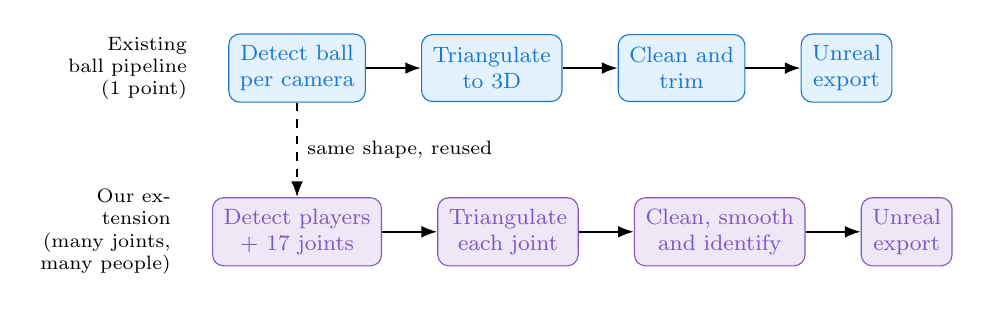
\begin{tikzpicture}[node distance=5mm and 7mm]
  % existing
  \node[nball] (b1) {Detect ball\\per camera};
  \node[nball, right=of b1] (b2) {Triangulate\\to 3D};
  \node[nball, right=of b2] (b3) {Clean and\\trim};
  \node[nball, right=of b3] (b4) {Unreal\\export};
  \draw[flow] (b1)--(b2); \draw[flow] (b2)--(b3); \draw[flow] (b3)--(b4);
  \node[left=4mm of b1, font=\scriptsize, align=right, text width=1.7cm] {Existing\\ball pipeline\\(1 point)};
  % ours
  \node[nours, below=12mm of b1] (u1) {Detect players\\+ 17 joints};
  \node[nours, right=of u1] (u2) {Triangulate\\each joint};
  \node[nours, right=of u2] (u3) {Clean, smooth\\and identify};
  \node[nours, right=of u3] (u4) {Unreal\\export};
  \draw[flow] (u1)--(u2); \draw[flow] (u2)--(u3); \draw[flow] (u3)--(u4);
  \node[left=4mm of u1, font=\scriptsize, align=right, text width=1.7cm] {Our extension\\(many joints,\\many people)};
  \draw[flowd] (b1) -- node[font=\scriptsize, right] {same shape, reused} (u1);
\end{tikzpicture}
\caption{The existing single-point ball pipeline (top) and the Group 1 extension to many players
and many joints (bottom). The processing shape is reused; the data is generalised.}
\label{fig:ballvsours}
\end{center}
\end{figure}

\section{Phase 0: foundation readiness}
The purpose of Phase 0 is to prove the ground is solid before any model code is written: that
the data is complete and synchronised, that the calibration files load and behave correctly, and
that the output format handed to Groups 2 and 3 is agreed and frozen. Skipping this step risks a
missing frame, a broken calibration file, or a vague handoff format surfacing weeks later as a
confusing bug.

The method is an automated readiness audit that performs the four checks in
Table~\ref{tab:phase0}, each of which writes a compact evidence file. The audit deliberately
separates two questions: whether the engineering is sound, and whether the management-level
decisions that sit outside the code (for example who owns the validation data and what accuracy
counts as passing) have been resolved.

\begin{table}[!h]
	\begin{center}
		\caption{The four checks performed by the Phase 0 readiness audit.}
		\label{tab:phase0}
		\footnotesize
		\begin{tabular}{p{3.0cm}p{11.0cm}}
			\toprule
			\textbf{Check} & \textbf{What it proves} \\
			\midrule
			Dataset inventory & All 7 cameras present, 600 frames each, frame identifiers
			synchronised, correct 2560x1440 resolution. \\
			Calibration & Calibration files load, matrices are valid, surveyed points project
			correctly, and the existing ball reprojection is reproducible. \\
			Events pipeline & The existing ball artifact chain is present and its reprojection
			errors are summarised. \\
			Output contract & The JSON format to be delivered to Groups 2 and 3 is explicit and
			validates in code. \\
			\bottomrule
		\end{tabular}
	\end{center}
\end{table}

The output contract deserves emphasis. It fixes the structure of the data each downstream group
receives, with the identity, role, and 3D fields present as placeholders that later phases fill.
Freezing the contract early means Groups 2 and 3 can build against it in parallel, before the
later phases are complete. The full schema is given in Appendix~\ref{app:contract}.

\section{Phase 1: per-camera perception}
The purpose of Phase 1 is, for every camera and every frame, to find each person as a bounding
box and to estimate that person's 2D pose as seventeen body joints with a confidence score for
each. Three terms are used: a \emph{bounding box} is a rectangle around a detected person; the
\emph{2D pose} is the on-image position of the seventeen standard COCO joints (eyes, shoulders,
elbows, wrists, hips, knees, ankles, and so on); and \emph{confidence} is how sure the model is
about each joint, which later stages use to reject noise. The existing detector finds only the
ball, so detecting multiple players and their joints is net-new work and the front end on which
every later phase depends.

The method is a per-camera person detector and 2D pose stage built on YOLO26x-pose
\cite{ultralytics_pose}, run over the full delivery. This model was chosen first deliberately,
following the Week 1 to 2 shortlist: it is the fastest path to a working baseline, combining
detection and pose in a single model with easy GPU deployment and broad export. It is the
minimum-viable baseline, not the final choice. The run used a CUDA GPU at image size 640, batch
size 32, half precision (FP16), full-frame inference, with non-maximum-suppression IoU 0.7 and a
detection confidence threshold of 0.25. The results are reported in Chapter~\ref{ch:results}.

% =====================================================================
\chapter{Results and Discussions}
\label{ch:results}
% =====================================================================
This chapter reports the verified outcomes of the two completed phases on the real cricket
dataset, together with supporting evidence from the public-dataset benchmark, and then states
honestly the gap that the remaining phases must close.

\section{The cricket dataset}
Phase 0 confirmed the structure of the supplied capture, summarised in
Table~\ref{tab:dataset}. The seven cameras are calibrated into one shared world coordinate
system, which is what makes triangulation possible. Figure~\ref{fig:rig} shows the rig layout
and coordinate convention from the project's calibration reference.

\begin{table}[!h]
	\begin{center}
		\caption{The Phase 0 verified properties of the supplied cricket capture.}
		\label{tab:dataset}
		\footnotesize
		\begin{tabular}{p{3.2cm}p{10.8cm}}
			\toprule
			\textbf{Item} & \textbf{Detail} \\
			\midrule
			Cameras & 7 synchronised, calibrated cameras (camera01 to camera07) in three capture
			groups. \\
			Footage & 600 frames per camera per delivery; the worked delivery is 4{,}200 frames
			across the 7 cameras. \\
			Resolution & 2560 x 1440 pixels per frame. \\
			Calibration & Bundle-adjusted intrinsics and extrinsics, per-camera 3x4 projection
			matrices, and a pitch-plane configuration. \\
			Existing pipeline & A working ball-tracking chain that detects, triangulates, cleans,
			and exports a single point to Unreal. \\
			\bottomrule
		\end{tabular}
	\end{center}
\end{table}

\begin{figure}[ht]
\begin{center}
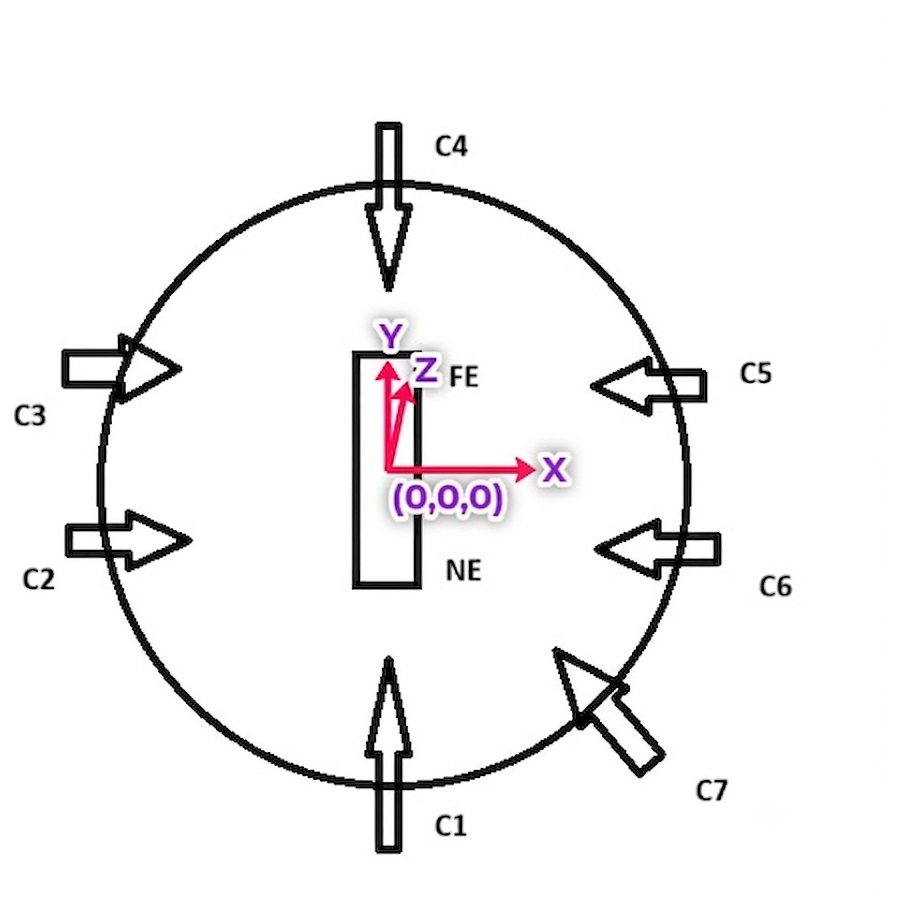
\includegraphics[width=0.58\textwidth]{figures/conventions_trim.jpeg}
\caption{The seven-camera rig and shared world-coordinate convention from the project's
calibration reference. The cameras ring the pitch and point inward; all are calibrated into a
single origin and axis system, which lets a joint seen in several cameras be triangulated into
one 3D point.}
\label{fig:rig}
\end{center}
\end{figure}

\section{Phase 0 result: technically complete, externally blocked}
The audit produced a clear and intentionally honest split. The internal status is a pass: all
technical checks are green, the calibration is usable, and the output contract validates in code.
The external status is blocked, with seven open items that are management decisions rather than
code gaps, for example the ownership of the validation dataset, who produces the manual
ground-truth labels, and what accuracy thresholds count as passing.
Figure~\ref{fig:phase0status} shows this split. These items were surfaced and escalated rather
than guessed, which is the correct engineering posture: the engineering side of Phase 0 is
complete, and the remaining items require a decision from the company.

\begin{figure}[ht]
\begin{center}
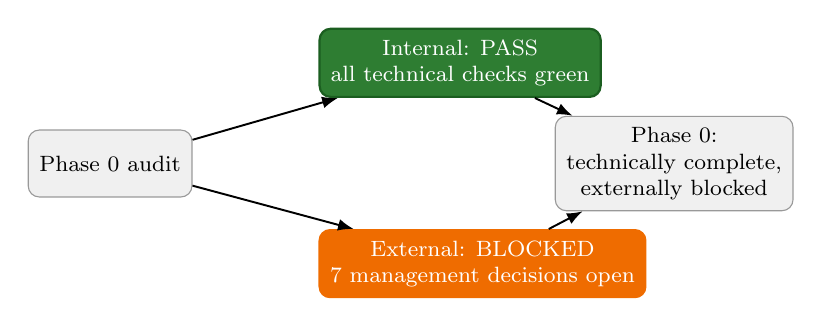
\begin{tikzpicture}[node distance=6mm and 12mm]
  \node[nneu] (a) {Phase 0 audit};
  \node[ndone, above right=4mm and 16mm of a] (b) {Internal: PASS\\all technical checks green};
  \node[fbox, fill=cwarn, text=white, draw=cwarn, below right=4mm and 16mm of a] (c) {External: BLOCKED\\7 management decisions open};
  \node[nneu, right=46mm of a] (d) {Phase 0:\\technically complete,\\externally blocked};
  \draw[flow] (a)--(b); \draw[flow] (a)--(c);
  \draw[flow] (b)--(d); \draw[flow] (c)--(d);
\end{tikzpicture}
\caption{Phase 0 outcome. All technical checks pass; the remaining items are escalated
management decisions, not code gaps. The output contract is frozen so Groups 2 and 3 can proceed
in parallel.}
\label{fig:phase0status}
\end{center}
\end{figure}

\section{Phase 1 result: per-camera detection and 2D pose}
Phase 1 produced per-camera person detections and 2D poses over the full delivery. The verified
run statistics are in Table~\ref{tab:phase1}. Across 4{,}200 frame records the stage produced
13{,}170 player detections with no empty or failed frames, at a median model inference time of
11.3 ms per frame.

\begin{table}[!h]
	\begin{center}
		\caption{Verified Phase 1 run statistics (run p1-yolo26x, full delivery, all 7 cameras).}
		\label{tab:phase1}
		\footnotesize
		\begin{tabular}{p{6.5cm}p{6.0cm}}
			\toprule
			\textbf{Metric} & \textbf{Value} \\
			\midrule
			Frame records written & 4{,}200 (600 x 7 cameras) \\
			Total player detections & 13{,}170 \\
			Median model inference & 11.3 ms per frame (p95: 20.7 ms) \\
			End-to-end speed (offline batch) & 16.6 FPS (including image decode and disk I/O) \\
			Empty or failed frames & 0 \\
			Status & pass \\
			\bottomrule
		\end{tabular}
	\end{center}
\end{table}

The number of detections per camera reflects how many players each view actually sees, shown in
Figure~\ref{fig:detbars}. The end-on bowler and field cameras see the most players, while the
tight side view (camera07) sees the fewest. The average number of players seen per frame ranged
from 5.0 in the field view down to 1.1 in the tight view, which is consistent with the camera
layout in Figure~\ref{fig:rig}.

\begin{figure}[ht]
\begin{center}
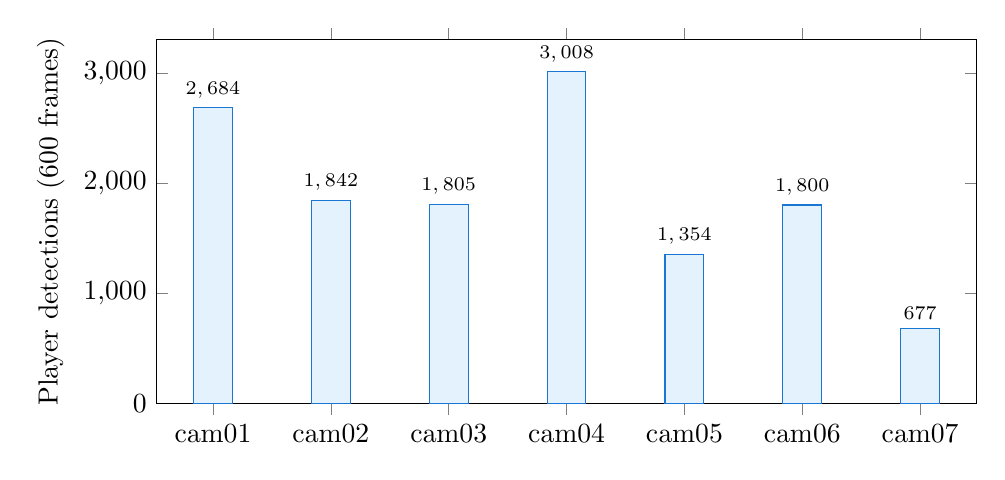
\begin{tikzpicture}
\begin{axis}[
  width=12cm, height=6.2cm,
  ybar, bar width=14pt,
  ymin=0, ymax=3300,
  ylabel={Player detections (600 frames)},
  symbolic x coords={cam01,cam02,cam03,cam04,cam05,cam06,cam07},
  xtick=data,
  nodes near coords, nodes near coords style={font=\scriptsize},
  every node near coord/.append style={/pgf/number format/1000 sep={,}},
  enlarge x limits=0.08,
]
  \addplot[draw=cballD, fill=cball] coordinates {
    (cam01,2684) (cam02,1842) (cam03,1805) (cam04,3008) (cam05,1354) (cam06,1800) (cam07,677)};
\end{axis}
\end{tikzpicture}
\caption{Total player detections per camera over 600 frames. The field view (camera04) sees the
most players and the tight side view (camera07) the fewest, consistent with the rig geometry.}
\label{fig:detbars}
\end{center}
\end{figure}

\section{Supporting evidence: public-dataset benchmark}
To anchor the chosen baseline against a standard reference, the same model was benchmarked
through the Week 3 repository on the full 5{,}000-image COCO 2017 keypoint validation set
\cite{lin2014coco}. YOLO26x-pose scored an OKS Average Precision of 0.710 (AP50 0.904, AP75
0.779) with an average recall of 0.771, at a median latency of 42.6 ms per image (batch size 8,
image size 640, single-precision). This run is recorded with full hardware and software
metadata in the repository. It is reported here as supporting evidence for the baseline's
accuracy on a public benchmark, and it is deliberately not compared directly against the cricket
run, because the protocol, precision, and batch settings differ.

\section{The honest gap}
The Phase 1 detections are correct, but watching the rendered overlay video makes three
limitations obvious, and these are exactly what the later phases exist to fix. First, the
skeletons jitter from frame to frame, because each frame is processed independently with no
temporal memory. Second, there are no identities: the same player is treated as a new detection
in every frame and in every camera. Third, there are no roles: the system does not know who is
the bowler, the striker, or the wicketkeeper. Figure~\ref{fig:gap} maps each limitation to the
phase that resolves it. This gap is the launch point for the second half of the project.

\begin{figure}[ht]
\begin{center}
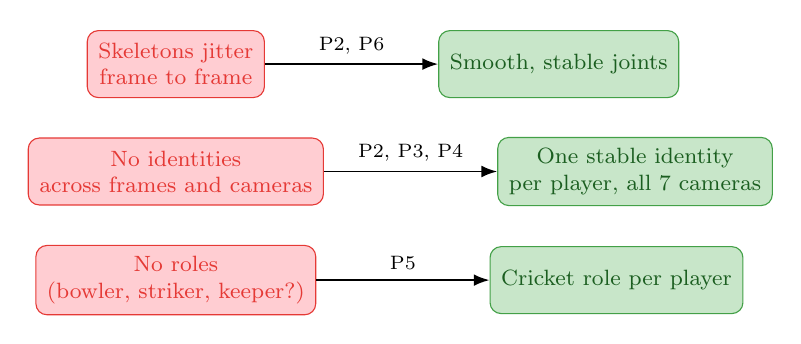
\begin{tikzpicture}[node distance=5mm and 22mm]
  \node[nprob] (n1) {Skeletons jitter\\frame to frame};
  \node[nprob, below=of n1] (n2) {No identities\\across frames and cameras};
  \node[nprob, below=of n2] (n3) {No roles\\(bowler, striker, keeper?)};
  \node[ngood, right=of n1] (g1) {Smooth, stable joints};
  \node[ngood, right=of n2] (g2) {One stable identity\\per player, all 7 cameras};
  \node[ngood, right=of n3] (g3) {Cricket role per player};
  \draw[flow] (n1) -- node[font=\scriptsize, above] {P2, P6} (g1);
  \draw[flow] (n2) -- node[font=\scriptsize, above] {P2, P3, P4} (g2);
  \draw[flow] (n3) -- node[font=\scriptsize, above] {P5} (g3);
\end{tikzpicture}
\caption{The honest gap after Phase 1. Detection works, but the output is jittery, identity-less,
and role-less. Each limitation maps to the later phase that resolves it.}
\label{fig:gap}
\end{center}
\end{figure}

% =====================================================================
\chapter{Conclusions and Future Work}
\label{ch:conclusions}
% =====================================================================

\section{Summary of the first four weeks}
The first four weeks established a solid, verified foundation. Weeks 1 and 2 framed the core
speed against accuracy trade-off, surveyed and audited more than fifty post-2020 pose models with
sourced numbers, and established the multi-camera triangulation path from 2D to 3D. Week 3 turned
that survey into a reproducible benchmarking repository with a single measurement protocol. Week
4 applied this foundation to real cricket data: Phase 0 passed all technical readiness checks and
froze the output contract, and Phase 1 produced verified per-camera detection and 2D pose over a
full delivery, with 13{,}170 detections across 4{,}200 frames and no failures. The work that
remains is to turn these correct but jittery, anonymous detections into clean, identified, smooth
3D motion.

\section{Phase 2: per-camera tracking (immediate next work)}
The immediate next phase gives each camera a memory of players over time. Phase 1 finds people
from scratch in every frame and has no notion that a person in one frame is the same person in
the next. Phase 2 links a player's detections across time within a single camera, so that the
same person keeps one stable local track identifier through movement and brief occlusion. The
output is a set of per-camera tracklets, where a tracklet is one person's continuous path through
that camera's frames. Figure~\ref{fig:tracking} shows the intended effect.

\begin{figure}[ht]
\begin{center}
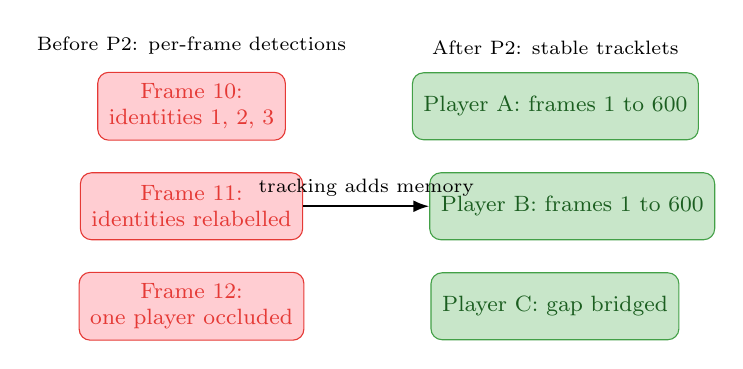
\begin{tikzpicture}[node distance=4mm and 16mm]
  \node[nprob] (b1) {Frame 10:\\identities 1, 2, 3};
  \node[nprob, below=of b1] (b2) {Frame 11:\\identities relabelled};
  \node[nprob, below=of b2] (b3) {Frame 12:\\one player occluded};
  \node[ngood, right=of b1] (a1) {Player A: frames 1 to 600};
  \node[ngood, right=of b2] (a2) {Player B: frames 1 to 600};
  \node[ngood, right=of b3] (a3) {Player C: gap bridged};
  \draw[flow] (b2) -- node[font=\scriptsize, above] {tracking adds memory} (a2);
  \node[font=\scriptsize, above=1mm of b1] {Before P2: per-frame detections};
  \node[font=\scriptsize, above=1mm of a1] {After P2: stable tracklets};
\end{tikzpicture}
\caption{Per-camera tracking turns relabelled per-frame detections into stable tracklets, each
following one player and bridging brief occlusion.}
\label{fig:tracking}
\end{center}
\end{figure}

The method is standard multi-object tracking adapted to the footage, matching each detection to
an existing track using three signals: a Kalman motion model \cite{kalman1960} that predicts
where a tracked player should next appear; a compact appearance embedding to confirm matches,
noting that identical kits limit how much appearance can contribute; and a geometry prior from
the calibrated cameras to gate matches by real-world plausibility. Several trackers will be
benchmarked on the project's own data through the Week 3 protocol, including DeepSORT
\cite{wojke2017deepsort} and the ByteTrack and BoT-SORT class
\cite{zhang2022bytetrack,aharon2022botsort}, alongside a geometry-assisted variant. The reported
measures will be the number of identity switches per delivery within a camera (lower is better)
and track completeness (the fraction of a player's true path that is followed). The exit
criterion is stable per-camera tracklets for a full delivery, with those numbers recorded; this
becomes the input to cross-camera re-identification in Phase 3.

\section{Roadmap: Phases 3 to 7}
The remaining phases combine the seven cameras, attach identities and roles, and produce smooth
3D for Unreal. They are distributed across the team as set out in Table~\ref{tab:roadmap}, which
states ownership only to make the plan concrete.

\begin{table}[!h]
	\begin{center}
		\caption{Roadmap of the remaining Group 1 phases.}
		\label{tab:roadmap}
		\footnotesize
		\begin{tabular}{p{1.4cm}p{10.6cm}p{1.8cm}}
			\toprule
			\textbf{Phase} & \textbf{In one sentence} & \textbf{Owner} \\
			\midrule
			P3 & Match the same physical player across all 7 views using geometry first
			(triangulation and reprojection, epipolar lines, and a ground-plane foot test), since
			kits are identical. & Teammate \\
			P4 & Collapse per-camera tracks and cross-camera matches into one stable global
			identity per player for the whole delivery, repairing identity switches and bridging
			occlusion. & Teammate \\
			P5 & Label each player with a cricket role (bowler, striker, non-striker, wicketkeeper,
			umpire, fielder) using pitch geometry, motion rules, and role priors. & Teammate \\
			P6 & Triangulate the joints into 3D and run a multi-stage cleanup so the skeleton is
			smooth enough to animate, then export to JSON and to Unreal Engine. & Teammate \\
			P7 & Measure association accuracy, identity switches, and role accuracy on a blind
			dataset, and deliver the final reports and handover. & Teammate \\
			\bottomrule
		\end{tabular}
	\end{center}
\end{table}

The key idea in Phase 3 is to lead with geometry rather than appearance. Because both teams wear
near-identical kits, appearance-based matching is unreliable. Instead, if a player seen in one
camera and a player seen in another triangulate to the same point in the real world, and their
feet land on the same spot on the pitch, they are the same person. This reuses the exact
reprojection check already proven in the ball pipeline.

\section{The smoothness problem (Phase 6 preview)}
The hardest part of the whole mandate is making the 3D skeleton smooth enough for Unreal. Any
residual jitter appears as a twitching limb on broadcast. Multi-view triangulation is inherently
jittery: one noisy joint, one missing camera, or one bad line of sight can make a 3D joint jump
between frames. The planned answer is a staged cleanup pipeline in which each known noise source
is removed by a specific stage, as mapped in Table~\ref{tab:noise} and sequenced in
Figure~\ref{fig:noise}.

\begin{table}[!h]
	\begin{center}
		\caption{Noise sources in multi-view 3D reconstruction and the stage that removes each.}
		\label{tab:noise}
		\footnotesize
		\begin{tabular}{p{6.0cm}p{8.0cm}}
			\toprule
			\textbf{Noise source} & \textbf{Removed by} \\
			\midrule
			2D keypoint jitter & A. Confidence gating and D. Temporal smoothing \\
			Triangulation outliers (one bad ray) & A. RANSAC ray rejection \cite{fischler1981ransac}
			and C. Reprojection-error rejection \\
			Missing views or occlusion & B. Confidence-weighted triangulation and F. inverse
			kinematics fill \\
			Reprojection error (calibration slack) & C. Reprojection-error rejection \\
			Bone-length drift & E. Skeleton constraints (constant bone length) \\
			Foot-skate (feet sliding) & F. Inverse kinematics and foot-lock \\
			Rotation jitter & G. Quaternion SLERP rotation smoothing \cite{shoemake1985slerp} \\
			\bottomrule
		\end{tabular}
	\end{center}
\end{table}

\begin{figure}[ht]
\begin{center}
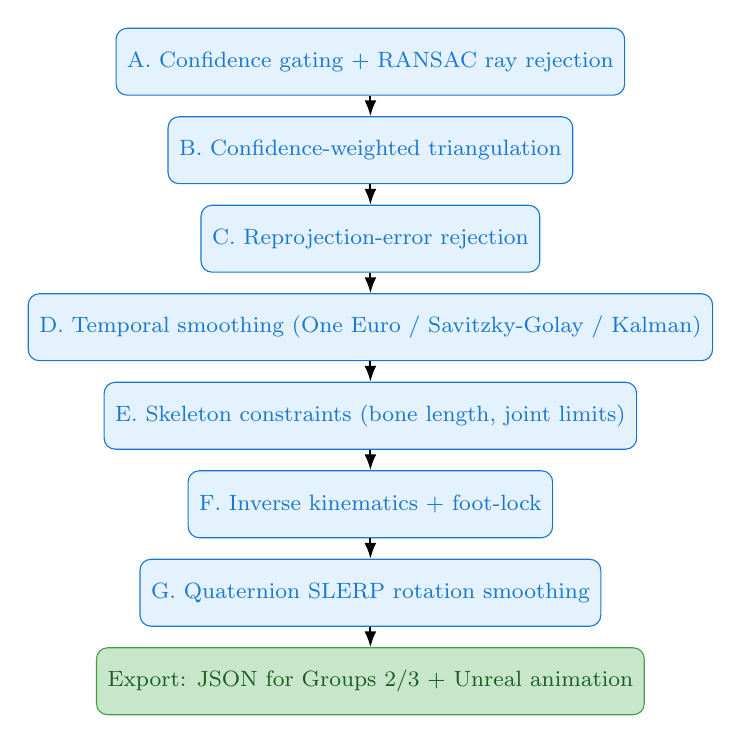
\begin{tikzpicture}[node distance=2.6mm]
  \node[nstep] (a) {A. Confidence gating + RANSAC ray rejection};
  \node[nstep, below=of a] (b) {B. Confidence-weighted triangulation};
  \node[nstep, below=of b] (c) {C. Reprojection-error rejection};
  \node[nstep, below=of c] (d) {D. Temporal smoothing (One Euro / Savitzky-Golay / Kalman)};
  \node[nstep, below=of d] (e) {E. Skeleton constraints (bone length, joint limits)};
  \node[nstep, below=of e] (f) {F. Inverse kinematics + foot-lock};
  \node[nstep, below=of f] (g) {G. Quaternion SLERP rotation smoothing};
  \node[ngood, below=of g] (x) {Export: JSON for Groups 2/3 + Unreal animation};
  \foreach \p/\q in {a/b,b/c,c/d,d/e,e/f,f/g,g/x} \draw[flow] (\p)--(\q);
\end{tikzpicture}
\caption{The planned staged cleanup pipeline. Raw, jittery, anonymous detections enter and one
clean, identified, smooth 3D skeleton leaves, ready for broadcast
\cite{casiez2012oneeuro,savitzky1964golay}.}
\label{fig:noise}
\end{center}
\end{figure}

\section{Concluding remarks}
The first half of the Practice School delivered a verified foundation rather than a premature end
to end demonstration: an audited model survey, a reproducible benchmarking framework, a passing
foundation audit, and a working per-camera perception stage on real cricket data. The honest
assessment is that the detections are correct but not yet stable, identified, or three
dimensional. The plan for the second half is concrete and dependency-ordered, beginning with
per-camera tracking and progressing through geometry-first cross-camera association, role
assignment, and staged 3D cleanup toward the smooth, identified output that the broadcast stories
and Unreal Engine rendering require.

% =====================================================================
\chapter{Recommendations}
\label{ch:recommendations}
% =====================================================================
The following recommendations follow from the audited survey and the Week 4 results.

\paragraph{Match the model to the use case.} No single pose model is best for every job. The
survey supports the use-case-driven shortlist in Table~\ref{tab:reco}: a whole-body model for
balanced cricket biomechanics, an occlusion-robust whole-body model for heavily obscured joints,
a one-stage body model for real-time multi-player tracking, and a fast, broadly exportable model
for a first deployment. The Week 4 baseline deliberately started from the last of these and
should be revisited against the others once tracking and association are in place.

\begin{table}[!h]
	\begin{center}
		\caption{Use-case-driven model recommendations from the survey.}
		\label{tab:reco}
		\footnotesize
		\begin{tabular}{p{4.4cm}p{3.0cm}p{6.6cm}}
			\toprule
			\textbf{Use case} & \textbf{Recommended model} & \textbf{Reason} \\
			\midrule
			Balanced overall & RTMW-x / RTMW-l & Whole-body detail plus practical speed; fits
			cricket biomechanics. \\
			Heavy occlusion & DWPose-l & Explicitly trained to infer hidden joints (bat, pads,
			gloves). \\
			Real-time, many players & RTMO-l & One-stage; cost independent of player count; strong
			under crowding. \\
			Fast first deployment & YOLO26x-pose & Quick to ship, broad export support, good
			enough accuracy. \\
			\bottomrule
		\end{tabular}
	\end{center}
\end{table}

\paragraph{Lead with geometry, not appearance.} Because the two teams wear near-identical kits,
cross-camera matching and 3D cleanup should rely first on the calibrated camera geometry, with
appearance used only as a tie-breaker. This reuses the proven ball-pipeline reprojection check
and is more robust than appearance-only association.

\paragraph{Keep every experiment reproducible.} All future model and tracker comparisons should
run through the Week 3 benchmarking protocol, with full hardware and software metadata recorded,
so that results remain comparable across people and machines. Speed conclusions should be drawn
only from appropriate GPU hardware, not from laptops.

\paragraph{Escalate the open management decisions early.} The remaining Phase 0 blockers, namely
ground-truth ownership, annotation tooling, and the validation accuracy targets, are decisions
rather than code. Resolving them early is necessary before the validation in Phase 7 can produce
meaningful numbers, and obtaining additional match data would strengthen any generalisation
claims, since the current work uses a single match.

% =====================================================================
\bibliography{ref}
\addcontentsline{toc}{chapter}{Bibliography}

% =====================================================================
\begin{appendices}

\chapter{Group 1 output contract schema}
\label{app:contract}
The frozen output contract delivered to Groups 2 and 3 uses the schema
identifier \texttt{g1\_\allowbreak player\_\allowbreak frame/\allowbreak v0} with the COCO-17
skeleton. The identity, role, and 3D fields are
present as placeholders that later phases fill, which lets the downstream groups build against
the format in parallel.

\begin{verbatim}
{
  "camera_id": "cam_01",
  "frame_index": 212334,
  "players": [{
    "bbox_xywh_px": [x, y, w, h],          // filled in Phase 1
    "pose_2d": {
      "keypoints_px": [ ... 17 ],          // filled in Phase 1
      "confidence":   [ ... 17 ]           // filled in Phase 1
    },
    "global_player_id": null,              // filled in Phase 4
    "role": "unknown",                     // filled in Phase 5
    "pose_3d": null                        // filled in Phase 6
  }]
}
\end{verbatim}

The role field takes one of the values bowler, striker, non\_striker, wicketkeeper, umpire,
fielder, or unknown.

\chapter{Extended model comparison}
\label{app:models}
Table~\ref{tab:extended} gives a wider slice of the audited survey. All figures are drawn from
official papers, repositories, or model cards, and accuracy figures are only comparable within the
same benchmark protocol (COCO-17, COCO-WholeBody-133, or the Sapiens v2 308-keypoint test).

\begin{table}[!h]
	\begin{center}
		\caption{Extended comparison of representative post-2020 pose models.}
		\label{tab:extended}
		\footnotesize
		\begin{tabular}{p{2.6cm}p{2.4cm}p{2.7cm}p{2.0cm}p{3.0cm}}
			\toprule
			\textbf{Model} & \textbf{Type} & \textbf{Accuracy} & \textbf{Size} & \textbf{Notes} \\
			\midrule
			RTMPose-m \cite{jiang2023rtmpose} & 2D body & 74.6 COCO AP & 13.6M & 430+ FPS on GTX
			1660 Ti. \\
			RTMPose-l \cite{jiang2023rtmpose} & 2D body & 75.8 COCO AP & 27.7M & TensorRT-FP16 3.46
			ms per crop. \\
			RTMO-m \cite{lu2023rtmo} & 2D body, one-stage & 70.9 COCO AP & 22.6M & about 81 FPS on
			V100. \\
			RTMO-l \cite{lu2023rtmo} & 2D body, one-stage & 74.8 AP; CrowdPose-Hard 65.3 & 44.8M &
			141 FPS on V100; strong occlusion behaviour. \\
			ViTPose-B \cite{xu2022vitpose} & 2D body, transformer & 75.8 COCO AP & 86M & 944 FPS on
			A100 (batch 64). \\
			ViTPose-H \cite{xu2022vitpose} & 2D body, transformer & 79.1 COCO AP & 632M & Accuracy
			ceiling for 2D body. \\
			DWPose-l \cite{yang2023dwpose} & 2D whole-body & 66.5 Whole AP (384x288) & about 4.5M &
			Distilled to infer hidden joints. \\
			RTMW-l \cite{jiang2024rtmw} & 2D whole-body & 70.1 Whole AP (384x288) & mid-size &
			Whole-body detail with practical speed. \\
			RTMW-x \cite{jiang2024rtmw} & 2D whole-body & 70.2 Whole AP (384x288) & mid-size & Best
			whole-body balance in the survey. \\
			Sapiens-1B \cite{khirodkar2024sapiens} & 2D dense whole-body & 72.7 Whole AP & 1.17B &
			Near-offline high-resolution analytics. \\
			Sapiens-2B \cite{khirodkar2024sapiens} & 2D dense whole-body & 74.4 Whole AP & 2.16B &
			Highest open whole-body accuracy. \\
			Sapiens2-1B \cite{sapiens2repo} & 2D dense (308 kpt) & 80.4 mAP (308-kpt test) & 1.46B
			& Separate 308-keypoint protocol; not comparable to COCO. \\
			YOLO11x-pose \cite{ultralytics_pose} & 2D body & 69.5 COCO AP & 58.8M & 82.6 FPS on T4. \\
			YOLO26x-pose \cite{ultralytics_pose} & 2D body & 71.6 COCO AP & 57.6M & Week 4 baseline;
			broad export support. \\
			BlazePose Heavy \cite{bazarevsky2020blazepose} & 2D + relative 3D & task-specific PCK &
			about 26 MB & On-device, single-person fitness tracking. \\
			\bottomrule
		\end{tabular}
	\end{center}
\end{table}

\end{appendices}

\end{document}
